\documentclass{scrreprt}

\usepackage{aligned-overset}
\usepackage{amsmath}
\usepackage{amssymb}
\usepackage{bm}
\usepackage[shortlabels]{enumitem}
\usepackage{hyperref}
\usepackage[utf8]{inputenc}
\usepackage{multicol}
\usepackage{mathtools}
\usepackage{physics}
\usepackage{tabularx}
\usepackage[table]{xcolor}
\usepackage{titling}
\usepackage{fancyhdr}
\usepackage{xfrac}
\usepackage{pgfplots}

\pgfplotsset{compat = newest}
\usetikzlibrary{intersections}
\usetikzlibrary{patterns}
\usepgfplotslibrary{fillbetween}

\author{Karsten Lehmann}
\date{WiSe 2021/2022}
\title{Übungsblatt 02\\Lineare Algebra - Grundlegende Konzepte}

\setlength{\headheight}{26pt}
\pagestyle{fancy}
\fancyhf{}
\lhead{\thetitle}
\rhead{\theauthor}
\lfoot{\thedate}
\rfoot{Seite \thepage}

\newcommand\ccg[1]{\cellcolor{green}{#1}}

\begin{document}
\paragraph{Aufgabe 2} Gegeben ist das gleichseitige Dreieck:

\begin{tikzpicture}
  \node[below left] at (0, 0) {A};
  \node[below right] at (3, 0) {B};
  \node[above] at (1.5, 2.598) {C};
  \draw[thick] (0, 0) -- (3, 0) -- (1.5, 2.598) -- cycle;
\end{tikzpicture} \\
Die Drehung des gegebenen Dreiecks gegen den Uhrzeigersinn um den Mittelpunkt
um $120^{\circ}$ (bzw. um $240^{\circ}$, bzw. um $360^{\circ}$) bezeichnen wir
mit $r_1$ (bzw. mit $r_2$, bzw. mit id). \\
Die Spiegelung des Dreiecks an den Höhen durch die Eckpunkte $A$, $B$ und $C$
werden mit $s_1$, $s_2$ und $s_3$ bezeichnet.

Man kann alle genannten Drehungen und Spiegelungen als Abbildungen auffassen -
somit kann man auch Kompositionen dieser betrachten. \\
Sei $D_6 \coloneqq \qty\big{\text{id}, r_1, r_2, r_3, s_1, s_2, s_3}$.

\begin{enumerate}[(1)]
\item \label{sec:2_1}
  Zeigen Sie, dass $D_6$ mit der Komposition von Abbildungen $\circ$ eine
  nicht-abelsche Gruppe ist.
  Stellen Sie die Gruppe $\qty\big(D_6, \circ)$ mithilfe einer
  Multiplikationstafel dar.

  \subparagraph{Lsg.} \underline{Multiplikationstabelle:} \\
  \begin{tabular}{c|>{\columncolor{yellow}}cccccc}
    $\circ$             & id       & $r_1$    & $r_2$       & $s_1$       & $s_2$       & $s_3$ \\
    \hline
    \rowcolor{yellow}id & \ccg{id} & $r_1$    & $r_2$       & $s_1$       & $s_2$       & $s_3$ \\
    $r_1$               & $r_1$    & $r_2$    & \ccg{id}    & $s_3$       & $s_1$       & $s_2$ \\
    $r_2$               & $r_2$    & \ccg{id} & $r_1$       & $s_2$       & $s_3$       & $s_1$ \\
    $s_1$               & $s_1$    & $s_3$    & $s_2$       & \ccg{id}    & $r_1$       & $r_2$ \\
    $s_2$               & $s_2$    & $s_1$    & $s_3$       & $r_2$       & \ccg{id}    & $r_1$ \\
    $s_3$               & $s_3$    & $s_2$    & $s_1$       & $r_1$       & $r_2$       & \ccg{id} \\
  \end{tabular} \\
  Nun heißt $\qty\big(D_6, \circ)$ eine Gruppe, falls
  \begin{enumerate}[(i)]
  \item Für $a, b, c \in D_6$ gilt
   $\qty\big(a \circ b) \circ c = a \circ \qty\big(b \circ c)$
    (\emph{Assoziativität}).
  \item ein \emph{neutrales Element} $e \in D_6$ existiert, sodass für jedes
    $a \in D_6$ gilt $e \circ a = a \circ e = a$.
    Das neutrale Element in $D_6$ ist \colorbox{yellow}{``id''}.
  \item für jedes Element $a \in D_6$ ein \emph{inverses Element}
    $a^{-1} \in D_6$ existiert mit \\
    \colorbox{green}{$a \circ a^{-1} = e =$ id}.
  \end{enumerate}

  \newpage
  Die Gruppe $\qty\big(D_6, \circ)$ heißt zusätzlich eine kommutative oder
  abelsche Gruppe, falls für $a, b \in D_6$ gilt $a \circ b = b \circ a$.
  Sei nun $a = s_2$ und $b = s_3$.
  Dann ergibt $b \circ a$:

  \begin{tikzpicture}
    \node[below left] at (0, 0) {A};
    \node[below right] at (1, 0) {B};
    \node[above] at (0.5, 0.866) {C};
    \draw[thick] (0, 0) -- (1, 0) -- (0.5, 0.866) -- cycle;
    \draw[black!60!green] (-0.5, 1) -- (1, 0);

    \node at (2.5, 0.4) {$\overset{{\color{black!60!green}\text{Spiegelung an $s_2$}}}\Rightarrow$};

    \node[below left] at (4, 0) {C};
    \node[below right] at (5, 0) {B};
    \node[above] at (4.5, 0.866) {A};
    \draw[thick] (4, 0) -- (5, 0) -- (4.5, 0.866) -- cycle;
    \draw[blue] (4.5, 0.866) -- (4.5, -0.866);

    \node at (6.5, 0.4) {$\overset{{\color{blue}\text{Spiegelung an $s_3$}}}\Rightarrow$};

    \node[below left] at (8, 0) {B};
    \node[below right] at (9, 0) {C};
    \node[above] at (8.5, 0.866) {A};
    \draw[thick] (8, 0) -- (9, 0) -- (8.5, 0.866) -- cycle;
  \end{tikzpicture} \\
  und $a \circ b$: \\
  \begin{tikzpicture}
    \node[below left] at (0, 0) {A};
    \node[below right] at (1, 0) {B};
    \node[above] at (0.5, 0.866) {C};
    \draw[thick] (0, 0) -- (1, 0) -- (0.5, 0.866) -- cycle;
    \draw[blue] (0.5, 0.866) -- (0.5, -0.866);

    \node at (2.5, 0.4) {$\overset{{\color{blue}\text{Spiegelung an $s_3$}}}\Rightarrow$};

    \node[below left] at (4, 0) {B};
    \node[below right] at (5, 0) {A};
    \node[above] at (4.5, 0.866) {C};
    \draw[thick] (4, 0) -- (5, 0) -- (4.5, 0.866) -- cycle;
    \draw[black!60!green] (3.5, 1) -- (5, 0);

    \node at (6.5, 0.4) {$\overset{{\color{black!60!green}\text{Spiegelung an $s_2$}}}\Rightarrow$};

    \node[below left] at (8, 0) {C};
    \node[below right] at (9, 0) {A};
    \node[above] at (8.5, 0.866) {B};
    \draw[thick] (8, 0) -- (9, 0) -- (8.5, 0.866) -- cycle;
  \end{tikzpicture} \\
  $\Rightarrow a \circ b \ne b \circ a$ \\
  $\Rightarrow \qty\big(D_6, \circ)$ ist eine nicht-abelsche Gruppe.

\item Geben Sie das neutrale Element von der Gruppe $\qty\big(D_6, \circ)$ an.

  \subparagraph{Lsg,} Wie in der Multiplikationstafel in \hyperref[sec:2_1]{(1)}
  zu sehen ist \colorbox{yellow}{id} das neutrale Element der Gruppe, da für
  alle $a \in D_6$ gilt $a \circ \text{id} = \text{id} \circ a = a$.

\item Geben Sie für jedes Element von $D_6$ sein Inverses an.

  \subparagraph{Lsg.} Wie in der Multiplikationstafel in \hyperref[sec:2_1]{(1)}
  \colorbox{green!40}{hervorgehoben:}
  \begin{multicols}{2}
    \begin{itemize}
    \item $\text{id} \circ \text{id} = \text{id}$
    \item $r_1 \circ r_2 = \text{id}$
    \item $r_2 \circ r_1 = \text{id}$
    \item $s_1 \circ s_1 = \text{id}$
    \item $s_2 \circ s_3 = \text{id}$
    \item $s_2 \circ s_3 = \text{id}$
    \end{itemize}
  \end{multicols}

\item Zeigen Sie, dass $\qty\big{\text{id}, r_1, r_2}$ eine Untergruppe von
  $D_6$ ist.

  \subparagraph{Lsg.} Die Teilmenge $\qty\big{\text{id}, r_1, r_2} \subset D_6$
  wird Untergruppe von $D_6$ genannt, falls
  \begin{enumerate}[1)]
  \item $1_{D_6} \in \qty\big{\text{id}, r_1, r_2}$
    $\Rightarrow$ Das neutrale Element ``id'' ist in
    $\qty\big{\text{id}, r_1, r_2}$ enthalten.

  \item Für $a, b \in \qty\big{\text{id}, r_1, r_2}$ gilt
    $a \circ b \in \qty\big{\text{id}, r_1, r_2}$

     \begin{multicols}{3}
       \begin{itemize}
       \item $\text{id} \circ \text{id} = \text{id}$
       \item $\text{id} \circ r_1 = r_1$
       \item $\text{id} \circ r_2 = r_2$
       \item $r_1 \circ \text{id} = r_1$
       \item $r_1 \circ r_1 = r_2$
       \item $r_1 \circ r_2 = \text{id}$
       \item $r_2 \circ \text{id} = r_2$
       \item $r_2 \circ r_1 = \text{id}$
       \item $r_2 \circ r_2 = r_1$
       \end{itemize}
     \end{multicols}
  \item Für $a \in \qty\big{\text{id}, r_1, r_2}$ gilt
    $a^{-1} \in \qty\big{\text{id}, r_1, r_2}$. \\
    Es existiert für jedes Element ein Inverses, nämlich
    ``id'' für ``id'', $r_2$ für $r_1$ und $r_1$ für $r_2$.
  \end{enumerate}

\end{enumerate}
\end{document}